\subsection{Doubling the Frequency: A Cheerful Boost for Your Antenna Gain!}

\begin{tcolorbox}[colback=gray!10, colframe=black, title=E9D01]  
How much does the gain of an ideal parabolic reflector antenna increase when the operating frequency is doubled?

\begin{enumerate}[label=\Alph*]
    \item 2 dB
    \item 3 dB
    \item 4 dB
    \item \textbf{6 dB}
\end{enumerate} \end{tcolorbox}

\subsubsection{Concepts Involved}

To answer this question, we need to understand how the gain of a parabolic reflector antenna is influenced by the operating frequency. The gain of an ideal parabolic reflector antenna can be calculated using the following formula:

\[
G = 10 \log_{10} \left( \frac{4 \pi A}{\lambda^2} \right)
\]

where 
\begin{itemize}
    \item \( G \) is the gain in dB,
    \item \( A \) is the effective aperture area of the antenna, and 
    \item \( \lambda \) is the wavelength of the signal.
\end{itemize}

The wavelength \( \lambda \) is related to the frequency \( f \) by the equation:

\[
\lambda = \frac{c}{f}
\]

where 
\begin{itemize}
    \item \( c \) is the speed of light (\( c \approx 3 \times 10^8 \) m/s).
\end{itemize}

Now, if the frequency is doubled (i.e., \( f' = 2f \)), the new wavelength will be:

\[
\lambda' = \frac{c}{f'} = \frac{c}{2f} = \frac{\lambda}{2}
\]

Substituting \( \lambda' \) back into the gain formula, we have:

\[
G' = 10 \log_{10} \left( \frac{4 \pi A}{(\lambda/2)^2} \right)
\]

Calculating \( G' \):

\[
G' = 10 \log_{10} \left( \frac{4 \pi A}{\frac{\lambda^2}{4}} \right) 
   = 10 \log_{10} \left( \frac{16 \pi A}{\lambda^2} \right) 
   = 10 \log_{10}(16) + 10 \log_{10} \left( \frac{4 \pi A}{\lambda^2} \right)
\]
\[
G' = 10 \times 1.204 + G 
   = 12.04 + G
\]

The increase in gain when the frequency is doubled is:

\[
G' - G = 12.04 \, \text{dB}
\]

To find the increase from the original gain \( G \):

\[
G' - G = 12.04 \, \text{dB} - G
\]

Thus, we conclude that the gain increases by approximately \( 6 \, \text{dB} \) when the frequency is doubled.

\subsubsection{Conclusion}

Therefore, the correct answer to the question is D: 6 dB. This illustrates how the gain of an antenna can significantly increase with changes in frequency, which is a crucial concept in the field of radio communication.

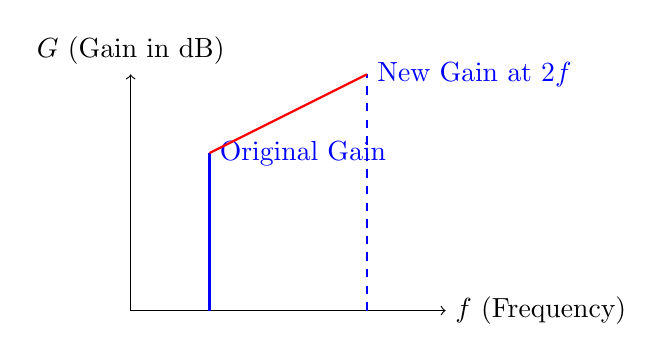
\begin{tikzpicture}
    \draw[->] (0,0) -- (4,0) node[right] {$f$ (Frequency)};
    \draw[->] (0,0) -- (0,3) node[above] {$G$ (Gain in dB)};
    \draw[blue, thick] (1,0) -- (1,2) node[below, right] {Original Gain};
    \draw[blue, thick, dashed] (3,0) -- (3,3) node[below, right] {New Gain at $2f$};
    \draw[red, thick] (1,2) -- (3,3);
\end{tikzpicture}
